\documentclass[aspectratio=169]{beamer}
\usetheme{Madrid}
\usecolortheme{default}

\usepackage{graphicx}
\usepackage{listings}
\usepackage{xcolor}
\usepackage{amsmath}
\usepackage{tikz}

\usepackage{url}

% Code listing setup
\lstset{
    basicstyle=\ttfamily\footnotesize,
    keywordstyle=\color{blue}\bfseries,
    commentstyle=\color{green!60!black},
    stringstyle=\color{red},
    breaklines=true,
    frame=single,
    backgroundcolor=\color{gray!10},
    language=Python
}

\title{Introduction to Dask}
\subtitle{Scalable Analytics in Python}
\author{CSE255 - Scalable Data Analysis}
\date{\today}

\begin{document}

\frame{\titlepage}

\begin{frame}{The Big Data Problem}
\begin{itemize}
    \item \textbf{Memory limits}: "What happens when data $>$ RAM?"
    \item Traditional tools (NumPy, Pandas) fail with large datasets
    \item Need for parallel and distributed computing
\end{itemize}

\vspace{0.5cm}
\begin{figure}[h]
    \centering
    % Draw a conceptual "data size vs. memory capacity" with TikZ
    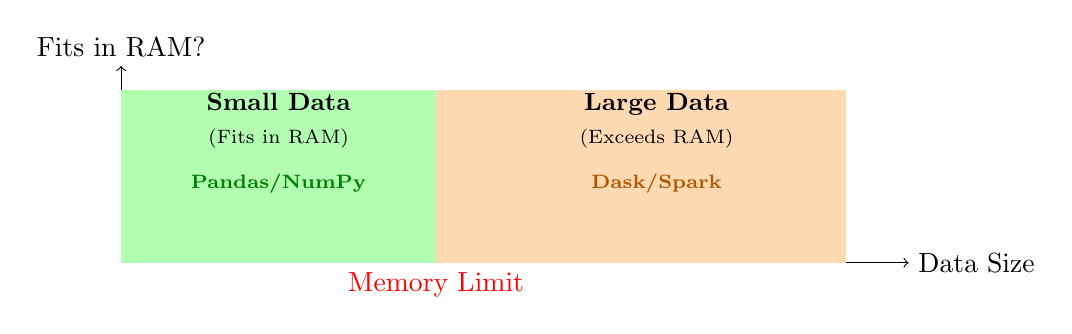
\begin{tikzpicture}[x=4cm, y=1cm]
        % Draw axes
        \draw[->] (0,0) -- (2.5,0) node[right] {Data Size};
        \draw[->] (0,0) -- (0,2.5) node[above] {Fits in RAM?};

        % Memory threshold line
        \draw[dashed,thick,color=red] (1,0) -- (1,2.2);
        \node[red,below] at (1,0) {Memory Limit};

        % Left: Small data zone
        \fill[green!30] (0,0) rectangle (1,2.2);
        \node[align=center] at (0.5,1.8) {\small\textbf{Small Data}\\\scriptsize(Fits in RAM)};
        \node[align=center,green!50!black] at (0.5,1.0) {\scriptsize\textbf{Pandas/NumPy}};

        % Right: Large data zone
        \fill[orange!30] (1,0) rectangle (2.3,2.2);
        \node[align=center] at (1.7,1.8) {\small\textbf{Large Data}\\\scriptsize(Exceeds RAM)};
        \node[align=center,orange!70!black] at (1.7,1.0) {\scriptsize\textbf{Dask/Spark}};

    \end{tikzpicture}

\end{figure}
\end{frame}

\begin{frame}{What is Dask?}
\begin{itemize}
    \item Parallel computing library for Python
    \item Scales from laptop to cluster
    \item Familiar APIs (NumPy-like, Pandas-like)
\end{itemize}
\end{frame}


\begin{frame}{Dask's Place in the Ecosystem}
\textbf{Tool Comparison:}

\vspace{0.3cm}
\begin{center}
\begin{tabular}{|l|p{3cm}|p{2cm}|p{3.5cm}|}
\hline
Tool & Scale & Language & Use Case \\
\hline
NumPy/Pandas & Single machine, in-memory & Python & Small-medium data \\
Dask & Single machine or cluster, larger-than-memory & Python & Large data, familiar APIs \\
Spark & Cluster & JVM (Scala/Java/Python) & Very large data, enterprise \\
\hline
\end{tabular}
\end{center}

\end{frame}

\begin{frame}{Why Dask?}
\begin{itemize}
    \item \textbf{Familiar APIs}: Works like pandas and NumPy
    \item \textbf{Pure Python}: No JVM required
    \item \textbf{Flexible}: Lazy evaluation enables optimization
    \item \textbf{Scalable}: From laptop to cluster
\end{itemize}

\vspace{0.5cm}
\textbf{Key Advantages:}
\begin{itemize}
    \item If you know pandas $\rightarrow$ you know Dask DataFrames
    \item If you know NumPy $\rightarrow$ you know Dask Arrays
    \item No need to learn new syntax
\end{itemize}
\end{frame}

\begin{frame}[fragile]{Core Concept: Lazy Evaluation}
\begin{itemize}
    \item Build computation graph first
    \item Execute only when needed (\texttt{.compute()})
    \item Enables optimization by scheduler
\end{itemize}

\vspace{0.3cm}
\textbf{Example:}
\begin{lstlisting}
df = dd.read_csv('data/*.csv')  # No data loaded yet
result = df.groupby('col').sum()  # Still no data loaded
final = result.compute()  # NOW data is loaded and processed
\end{lstlisting}

\vspace{0.2cm}
\begin{center}
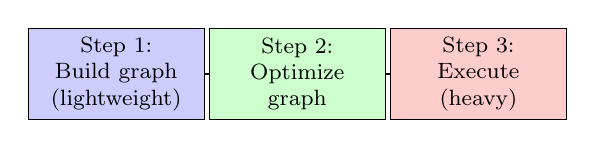
\begin{tikzpicture}[node distance=1.5cm, auto, scale=0.85, every node/.style={font=\footnotesize}]
    % Step 1: Build graph
    \node[draw, rectangle, fill=blue!20, text width=2cm, align=center] (build) {Step 1:\\Build graph\\(lightweight)};
    
    % Arrow
    \draw[->, thick] (build.east) -- ++(0.3,0);
    
    % Step 2: Optimize
    \node[draw, rectangle, fill=green!20, text width=2cm, align=center, right of=build, xshift=0.8cm] (optimize) {Step 2:\\Optimize graph};
    
    % Arrow
    \draw[->, thick] (optimize.east) -- ++(0.3,0);
    
    % Step 3: Execute
    \node[draw, rectangle, fill=red!20, text width=2cm, align=center, right of=optimize, xshift=0.8cm] (execute) {Step 3:\\Execute\\(heavy)};
\end{tikzpicture}
\end{center}
\end{frame}

\begin{frame}[fragile]{Task Graphs}
\begin{itemize}
    \item Dask builds graphs of operations
    \item \textbf{Nodes} = tasks (individual operations)
    \item \textbf{Edges} = dependencies (data flow)
    \item Scheduler optimizes execution order
\end{itemize}

\vspace{0.2cm}
\begin{center}
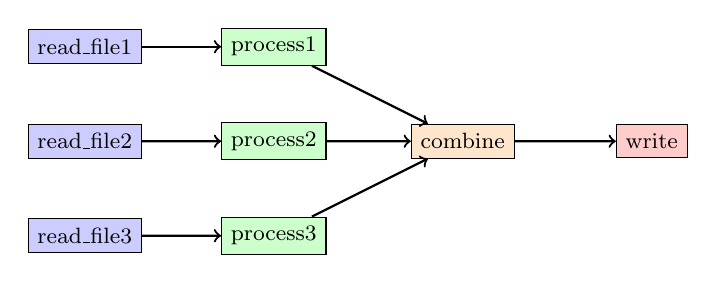
\begin{tikzpicture}[node distance=1.2cm, auto, scale=0.85, every node/.style={font=\footnotesize}]
    % Read nodes
    \node[draw, rectangle, fill=blue!20] (read1) {read\_file1};
    \node[draw, rectangle, fill=blue!20, below of=read1] (read2) {read\_file2};
    \node[draw, rectangle, fill=blue!20, below of=read2] (read3) {read\_file3};
    
    % Process nodes
    \node[draw, rectangle, fill=green!20, right of=read1, xshift=1.2cm] (proc1) {process1};
    \node[draw, rectangle, fill=green!20, right of=read2, xshift=1.2cm] (proc2) {process2};
    \node[draw, rectangle, fill=green!20, right of=read3, xshift=1.2cm] (proc3) {process3};
    
    % Combine node
    \node[draw, rectangle, fill=orange!20, right of=proc2, xshift=1.2cm] (combine) {combine};
    
    % Write node
    \node[draw, rectangle, fill=red!20, right of=combine, xshift=1.2cm] (write) {write};
    
    % Edges
    \draw[->, thick] (read1) -- (proc1);
    \draw[->, thick] (read2) -- (proc2);
    \draw[->, thick] (read3) -- (proc3);
    \draw[->, thick] (proc1) -- (combine);
    \draw[->, thick] (proc2) -- (combine);
    \draw[->, thick] (proc3) -- (combine);
    \draw[->, thick] (combine) -- (write);
\end{tikzpicture}
\end{center}
\end{frame}

\begin{frame}{Dask Collections Overview}
\textbf{Four Main Collections:}

\begin{enumerate}
    \item \textbf{DataFrame}: Many pandas DataFrames
    \begin{itemize}
        \item Tabular data, pandas-like API
    \end{itemize}
    
    \item \textbf{Array}: Many NumPy arrays
    \begin{itemize}
        \item N-dimensional arrays, NumPy-like API
    \end{itemize}
    
    \item \textbf{Bag}: Many Python objects
    \begin{itemize}
        \item Unstructured data, functional operations
    \end{itemize}
    
    \item \textbf{Delayed}: Arbitrary Python functions
    \begin{itemize}
        \item Custom workflows, general parallelization
    \end{itemize}

       \item \textbf{Futures}: Arbitrary Python functions
    \begin{itemize}
        \item Non-blocking distributed calculations. Latency minimization.
    \end{itemize}

\end{enumerate}
\end{frame}

\begin{frame}{Dask DataFrame = Many Pandas DataFrames}
\begin{itemize}
    \item One Dask DataFrame = collection of pandas DataFrames
    \item Partitioned along index
    \item Operations applied to each partition in parallel
\end{itemize}

\vspace{0.5cm}
\textbf{Key Points:}
\begin{itemize}
    \item Each partition is a real pandas DataFrame
    \item Partitions can be on different machines
    \item Operations happen in parallel across partitions
\end{itemize}

\vspace{0.2cm}
\begin{center}
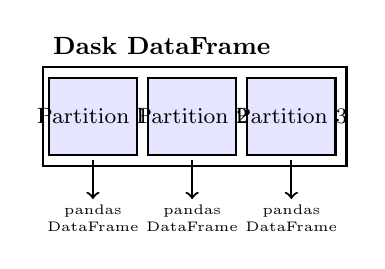
\begin{tikzpicture}[scale=0.7, every node/.style={font=\footnotesize}]
    % Draw DataFrame as a large rectangle
    \draw[thick] (0,0) rectangle (5.5,1.8) node[pos=.5] {};
    \node[anchor=south west, font=\small] at (0,1.85) {\textbf{Dask DataFrame}};
    
    % Draw partitions inside DataFrame
    \foreach \x/\label in {0/Partition 1, 1.8/Partition 2, 3.6/Partition 3} {
        \draw[fill=blue!10,thick] (\x+0.1,0.2) rectangle (\x+1.7,1.6);
        \node at (\x+0.9,0.9) {\label};
        \draw[->,thick] (\x+0.9,0.1) -- (\x+0.9,-0.6);
        \node[align=center, font=\tiny] at (\x+0.9,-0.95) {pandas\\DataFrame};
    }
\end{tikzpicture}
\end{center}

\end{frame}

\begin{frame}{When to Use Dask}
\textbf{Use Dask when:}
\begin{itemize}
    \item Data larger than memory (or close to it)
    \item Need parallel processing
    \item Want familiar pandas/NumPy APIs
    \item Need to scale beyond single machine
\end{itemize}

\vspace{0.5cm}
\textbf{Decision Tree:}
\begin{enumerate}
    \item Does data fit in memory? $\rightarrow$ No $\rightarrow$ Use Dask
    \item Need parallel processing? $\rightarrow$ Yes $\rightarrow$ Use Dask
    \item Want pandas-like API? $\rightarrow$ Yes $\rightarrow$ Use Dask DataFrame
\end{enumerate}
\end{frame}

\begin{frame}{When NOT to Use Dask}
\textbf{Don't use Dask when:}
\begin{itemize}
    \item Small datasets (use pandas/NumPy directly)
    \item Simple operations (overhead not worth it)
    \item Real-time processing (use streaming tools)
    \item Data fits comfortably in memory
\end{itemize}

\vspace{0.5cm}
\textbf{Rule of Thumb:}
\begin{itemize}
    \item If you have 5-10x RAM compared to dataset size $\rightarrow$ pandas is fine
    \item If dataset approaches or exceeds RAM $\rightarrow$ consider Dask
\end{itemize}
\end{frame}

\begin{frame}{Dask vs Alternatives}
\textbf{vs Pandas:}
\begin{itemize}
    \item Pandas: Single machine, in-memory
    \item Dask: Single machine or cluster, larger-than-memory, parallel
\end{itemize}

\vspace{0.3cm}
\textbf{vs Spark:}
\begin{itemize}
    \item Spark: JVM-based, cluster-focused, enterprise
    \item Dask: Python-native, flexible, easier to learn
\end{itemize}

\vspace{0.3cm}
\textbf{vs NumPy:}
\begin{itemize}
    \item NumPy: Single machine, in-memory arrays
    \item Dask: Single machine or cluster, larger arrays, distributed
\end{itemize}
\end{frame}

\begin{frame}[fragile]{Installation and Setup}
\textbf{Basic Installation:}
\begin{lstlisting}[language=bash]
pip install dask
\end{lstlisting}

\vspace{0.3cm}
\textbf{Complete Installation (recommended):}
\begin{lstlisting}[language=bash]
pip install dask[complete]
\end{lstlisting}

\vspace{0.3cm}
\textbf{For Distributed Computing:}
\begin{lstlisting}[language=bash]
pip install dask[distributed]
\end{lstlisting}

\vspace{0.3cm}
\textbf{What's Included:}
\begin{itemize}
    \item \texttt{dask[complete]}: All optional dependencies
    \item \texttt{dask[distributed]}: Distributed scheduler
    \item \texttt{dask[dataframe]}: DataFrame-specific dependencies
\end{itemize}
\end{frame}

\begin{frame}[fragile]{Basic Example}
\begin{lstlisting}
import dask.dataframe as dd

# Read data (lazy - no data loaded yet)
df = dd.read_csv('data/*.csv')

# Build computation (still lazy)
result = df.groupby('column').sum()

# Actually execute
result.compute()  # NOW data is loaded and processed
\end{lstlisting}

\vspace{0.3cm}
\textbf{What Happens:}
\begin{enumerate}
    \item \texttt{read\_csv()}: Creates task graph for reading files
    \item \texttt{groupby().sum()}: Adds grouping tasks to graph
    \item \texttt{compute()}: Executes all tasks in parallel
\end{enumerate}
\end{frame}

\begin{frame}{Summary}
\textbf{Key Takeaways:}
\begin{itemize}
    \item Dask = parallel computing for Python
    \item Familiar APIs (pandas, NumPy)
    \item Lazy evaluation for optimization
    \item Scales from laptop to cluster
\end{itemize}

\vspace{0.3cm}
\textbf{Next Steps:}
\begin{itemize}
    \item Learn Dask DataFrames (most common use case)
    \item Understand delayed and futures
    \item Explore distributed computing
\end{itemize}

\vspace{0.2cm}
\textbf{Core Concepts:}
\begin{itemize}
    \item Lazy evaluation
    \item Task graphs
    \item Partitioned collections
    \item Familiar APIs
\end{itemize}
\end{frame}

\end{document}

